\documentclass{article}
\title{An {\tt R} package for statistical provenance analysis}
\author{Pieter Vermeesch\footnote{
corresponding author: +44(0)2076792428, 
{\tt p.vermeesch@ucl.ac.uk}}\\ 
London Geochronology Centre, University College London, United Kingdom\\~\\
Alberto Resentini and Eduardo Garzanti\\
Laboratorio di Petrografia del Sedimentario, 
Universit\`{a} Milano-Bicocca, Italy}
\usepackage{graphicx,natbib,amsmath}
\begin{document}

\maketitle

\begin{abstract}
This paper introduces {\tt provenance}, a software package within the
statistical programming environment {\tt R}, which aims to facilitate
the visualisation and interpretation of large amounts of sedimentary
provenance data, including mineralogical, petrographic, chemical and
isotopic provenance proxies, or any combination of these. {\tt
  provenance} comprises functions to: (a) calculate the sample size
required to achieve a given detection limit; (b) plot distributional
data such as detrital zircon U-Pb age spectra as Cumulative Age
Distributions (CADs) or adaptive Kernel Density Estimates (KDEs); (c)
plot compositional data as pie charts or ternary diagrams; (d) correct
the effects of hydraulic sorting on sandstone petrography and heavy
mineral composition; (e) assess the settling equivalence of detrital
minerals and grain-size dependence of sediment composition; (f)
quantify the dissimilarity between distributional data using the
Kolmogorov-Smirnov and Sircombe-Hazelton distances, or between
compositional data using the Aitchison and Bray-Curtis distances; (e)
interpret multi-sample datasets by means of (classical and nonmetric)
Multidimensional Scaling (MDS) and Principal Component Analysis (PCA);
and (f) simplify the interpretation of multi-method datasets by means
of Generalised Procrustes Analysis (GPA) and 3-way MDS. All these
tools can be accessed through an intuitive query-based user interface,
which does not require knowledge of the {\tt R} programming
language. {\tt provenance} is free software released under the GPL-2
license and will be expanded based on user feedback.
\end{abstract}

\begin{center}
\emph{keywords: provenance -- statistics -- U-Pb -- zircon -- heavy
  minerals -- petrography -- geochemistry}
\end{center}

\section{Introduction}
\label{sec:intro}

Sedimentary provenance analysis, in which chemical, mineralogical and
isotopic properties of siliciclastic sediments are used to trace the
flow of sand (or silt) through a sediment routing system, has entered
an era of `Big Data' \citep{vermeesch2015}. Thanks to technological
improvements, it is now common practice to analyse thousands of grains
in dozens of samples. These large datasets can be prohibitively
difficult to interpret without statistical aids. Over the past few
years, sedimentary geologists and geochronologists have developed a
plethora of methods to address this issue, which are scattered in many
different places and implemented in a variety of different software
environments \citep[e.g.,][]{ludwig2003, marshall1996, sircombe2004a,
  sircombe2004b, resentini2013, templ2011, vandenboogaart2008,
  vermeesch2004b, vermeesch2012b, vermeesch2013, vermeesch2015}. This
paper aims to group some of the most useful tools under a common
umbrella, the {\tt provenance} package. The various sections of this
article are arranged in order of increasing complexity and
dimensionality, using a published dataset from Namibia for examples
(Section \ref{sec:datahandling}).

Section \ref{sec:singlesample} covers some functions that deal with a
single provenance proxy applied to a single sample of sediment.  This
includes sample size calculations (Section \ref{sec:samplesize}) and
functions to plot detrital age distributions as Kernel Density
Estimates and Cumulative Age Distributions (Section
\ref{sec:plotting}). Sections \ref{sec:srd} and \ref{sec:minsorting}
show how the effects of selective entrainment of dense minerals can be
undone and how mineralogical and petrographic provenance proxies are
affected by hydraulic sorting.  Section \ref{sec:multiplesamples}
introduces Principal Component Analysis and Multidimensional Scaling
as dimension reducing techniques which facilitate the interpretation
of multi-sample datasets analysed by a single method. This Section
also presents a brief overview of different approaches to quantify the
`dissimilarity' between distributional and compositional
data. Finally, section \ref{sec:multiplemethods} covers functionality
to combine large datasets comparing multiple samples analysed with
multiple methods, using Procrustes analysis and 3-way Multidimensional
Scaling. The various functions in this paper are illustrated with many
code snippets. Further examples are provided at {\tt
  http://provenance.london-geochron.com} and in the built-in
documentation. To run these examples and use the {\tt provenance}
package, one should first install {\tt R}. This is an increasingly
popular programming environment similar in scope and purpose to {\tt
  Matlab}, which is available free of charge on any operating system
at {\tt http://r-project.org}. The actual package can then be
installed by typing

\begin{verbatim}
install.packages('provenance')
\end{verbatim}

at the command prompt. Once installed, the package can be loaded by
typing

\begin{verbatim}
library(provenance)
\end{verbatim}

The easiest way to use {\tt provenance} is by typing:

\begin{verbatim}
provenance()
\end{verbatim}

which brings up a query-based user interface, removing the need to
master the syntax of the {\tt R} programming language (Figure
\ref{fig:gui}). The {\tt provenance()} user interface is self
explanatory and won't be discussed further in this paper.  Instead,
the different tools within the {\tt provenance} package will be
illustrated with short code snippets which more advanced users may
incorporate in their own {\tt R} scripts for enhanced flexibility and
automation. Internal documentation of these functions can be accessed
through the {\tt ?}  command.  For example, to display the
documentation for the {\tt procrustes} function (Section
\ref{sec:multiplemethods}):

\begin{verbatim}
?procrustes
\end{verbatim}

\begin{figure}
\centering
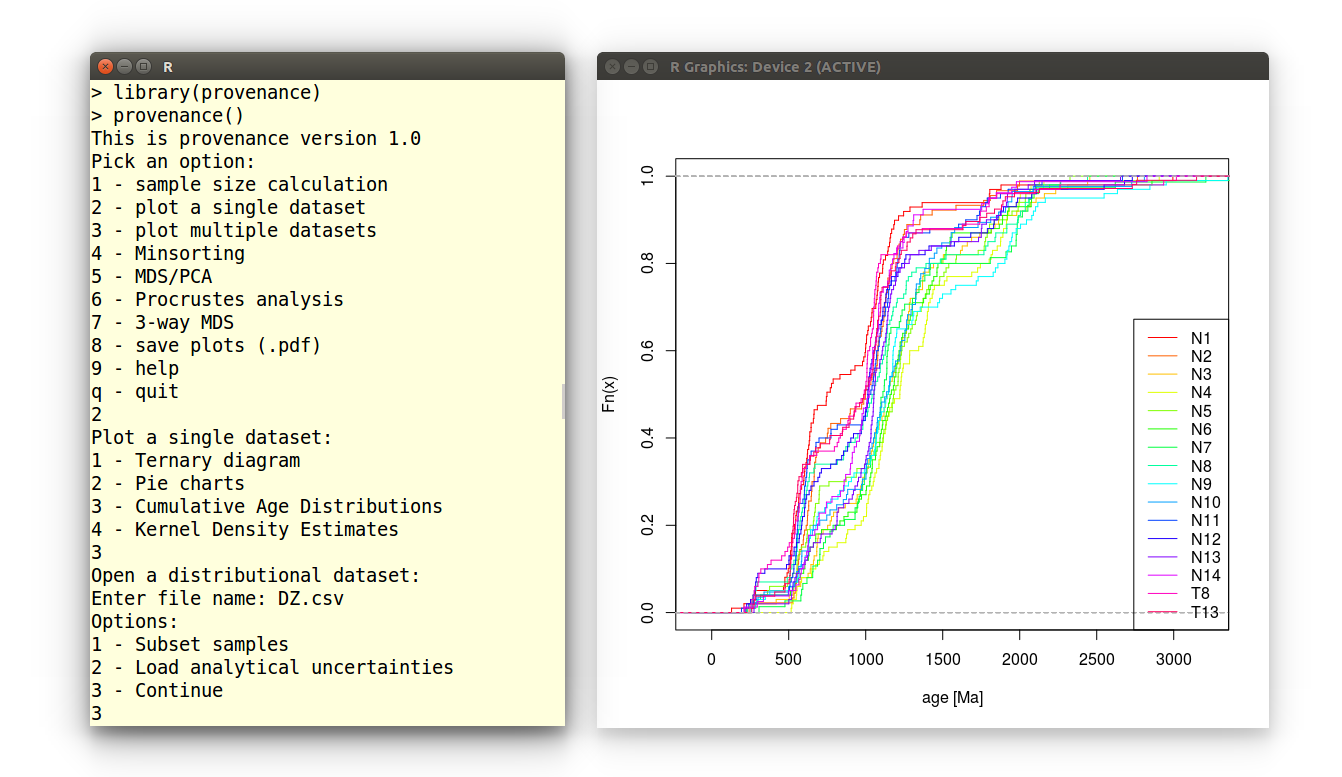
\includegraphics[width=\textwidth]{gui.png}
\caption{The query-based user interface.}
\label{fig:gui}
\end{figure}

\section{Data handling}
\label{sec:datahandling}

Over the years, geologists have tried and tested literally dozens of
provenance proxies \citep[e.g.,][]{basu1989, matter1985, morton1985,
  owen1987, renne1990, hurford1991, mclennan1993, vermeesch2015}. Most
of these can be diviced into two broad classes:

\begin{enumerate}
\item {\tt distributional} data cover single-mineral proxies such as
  detrital zircon U-Pb or mica $^{40}$Ar/$^{39}$Ar ages, in which
  samples can be summarised as lists of ordinal values.
\item {\tt compositional} data cover multi-mineral proxies such as
  petrography, heavy mineral analysis and bulk geochemistry, in which
  samples can be summarised as one-way tables in which each row can be
  (re)normalised to unity.
\end{enumerate}

{\tt provenance} reads raw data as {\tt .csv} files and casts these
into two classes by separate functions. For example:

\begin{verbatim}
DZ <- read.distributional(DZ.fname.csv,DZ.err.fname.csv)
HM <- read.compositional(HM.fname.csv)
\end{verbatim}

Here {\tt DZ.fname.csv} and {\tt DZ.err.fname.csv} stand for the
file names of some U-Pb age data and their analytical uncertainties
(where the latter argument is optional).  Different columns of these
files correspond to different samples, with the rows containing the
numerical values of the single grain analyses.  {\tt HM.fname.csv}
stands for the file name of a heavy mineral dataset, stored as a table
with samples arranged by row and each column corresponding to a
different type of mineral.  The data objects produced by the two
{\tt read} functions are treated differently by all subsequent
functions.

\subsection{Built-in datasets}
\label{sec:datasets}

To illustrate {\tt provenance}'s functionality, the package is bundled
with a published dataset from Namibia \citep{vermeesch2015}. Entering

\begin{verbatim}
data(Namib)
\end{verbatim}

loads a variable called {\tt Namib} into memory, which is comprised of
one distributional and five compositional datasets: (1) {\tt
  Namib\$DZ} contains the zircon U-Pb ages and their analytical
uncertainties; (2) {\tt Namib\$PT} the bulk petrography; (3) {\tt
  Namib\$HM} the heavy mineral compositions less the opaque minerals;
(4) {\tt Namib\$PTHM} the combined petrography and heavy minerals,
including micas and opaque minerals, normalised to unity; (5) {\tt
  Namib\$Major} the major element composition of the bulk sediment;
and (6) {\tt Namib\$Trace} the trace element composition of the bulk
sediment. To avoid having to repeatedly type the preamble {\tt
  Namib\$}, we can {\tt attach} the dataset to the search path:

\begin{verbatim}
attach(Namib)
\end{verbatim}

After which we can access its data members as {\tt DZ}, {\tt PT}
etc.  Additionally, {\tt provenance} also includes a table of mineral
and rock densities ({\tt densities}) as well as the
petrographic/mineralogical end-member compositions ({\tt endmembers})
of various tectonic settings which will be used to evaluate the
settling equivalence of detrital components (Section
\ref{sec:minsorting}). Also these two datasets can be loaded with the
{\tt data} function:

\begin{verbatim}
data(densities,endmembers)
\end{verbatim}

The built-in datasets are based on the following ten files: {\tt
  DZ.csv}, {\tt DZ.err.csv}, {\tt PT.csv}, {\tt HM.csv}, {\tt
  PTHM.csv}, {\tt Major.csv}, {\tt Trace.csv}, {\tt densities.csv} and
{\tt endmembers.csv}. The system paths of these files can be retrieved
as follows:

\begin{verbatim}
HM.fname.csv <- system.file("HM.csv",package="provenance")
\end{verbatim}

Further details about these datasets can be obtained from the built-in
help functions {\tt ?Namib}, {\tt ?densities} and
{\tt ?endmembers}.

\subsection{Basic data manipulation}
\label{sec:datamanipulation}

{\tt provenance} includes a number of basic operations to query and
manipulate the large datasets contained within {\tt distributional}
and {\tt compositional} data objects. For example, to extract the
coastal samples of the Namibian geochronology and heavy mineral
datasets:

\begin{verbatim}
coast.samples <- c('N1','N2','T8','T13','N12','N13')
coast.DZ <- subset(DZ,select=coast.samples)
coast.HM <- subset(HM,select=coast.samples)
\end{verbatim}

For compositional data, the {\tt subset} function also allows the
user to extract subcompositions. For example, to extract the zircon,
tourmaline and rutile content of all samples in the heavy mineral
dataset:

\begin{verbatim}
ZTR <- subset(HM,components=c('zr','tm','rt'))
\end{verbatim}

Of course, both options can also be combined:

\begin{verbatim}
coast.ZTR <- subset(HM,select=coast.samples,components=c('zr','tm','rt'))
\end{verbatim}

which returns the zircon, tourmaline and rutile contents of the
coastal samples alone. For compositional data, it is often useful to
add several components together, an operation which is referred to as
`amalgamation' \citep{aitchison1986}.  This is useful for removing
missing components (`zero counts') prior to logratio analysis (Section
\ref{sec:PCAMDS}). For example, to extract the QFL (Quartz -- Feldspar
-- Lithics) composition from the petrographic dataset by amalgamation:

\begin{verbatim}
QFL <- amalgamate(PT,Q='Q',F=c('KF','P'),L=c('Lm','Lv','Ls'))
\end{verbatim}

where {\tt KF} and {\tt P} stand for K-feldspar and plagioclase, and
{\tt Lm}, {\tt Lv} and {\tt Ls} refer to the lithic fragments of
metamorphic, volcanic and sedimentary origin respectively. In the
special case of a three component system, amalgamation can also be
achieved by a different function:

\begin{verbatim}
QFL.tern <- ternary(PT,'Q',c('KF','P'),c('Lm','Lv','Ls'))
\end{verbatim}

This produces an object of class {\tt ternary} which is handled by a
special, overloaded version of the {\tt plot} function (Section
\ref{sec:plotting}). The statistical field of compositional data
analysis is very rich, and {\tt provenance} does not attempt to cover
all but its most basic operations. The user is referred to other {\tt
  R} packages such as {\tt compositions} \citep{vandenboogaart2008}
and {\tt robCompositions} \citep{templ2011} for a more comprehensive
toolset. Three functions are provided to facilitate the interaction
between {\tt provenance} and these other packages.  {\tt as.acomp} and
{\tt as.data.frame} convert {\tt compositional} datasets to objects of
class {\tt acomp} and {\tt data.frame}, for use in {\tt
  robCompositions} and {\tt compositions}, repectively. For example:

\begin{verbatim}
PT.acomp <- as.acomp(PT)           # can be used in 'compositions'
PT.data.frame <- as.data.frame(PT) # can be used in 'robCompositions'
\end{verbatim}

Conversely, the {\tt as.compositional} function translates {\tt acomp}
or {\tt data.frame} objects to {\tt compositional} data for use in
{\tt provenance}. For example, using the {\tt Kongite} and {\tt
  skyeLavas} datasets which are built into {\tt compositions} and {\tt
  robCompositions}:

\begin{verbatim}
library(compositions)
data(Kongite)
Kongite.comp <- as.compositional(Kongite)
library(robCompositions)
data(skyeLavas)
skyeLavas.comp <- as.compositional(skyeLavas)
\end{verbatim}

where {\tt Kongite.comp} and {\tt skyeLavas.comp} can be further
analysed by the functions described later in this paper.

\section{Functions applying to a single sample}
\label{sec:singlesample}

\subsection{Sample size calculations}
\label{sec:samplesize}

On the most basic level, provenance analysis requires the geologist to
identify certain properties in a representative number of grains from
each sample. The question then arises how many grains constitute a
`representative' number of grains. The answer to this question depends
on the geological problem of interest. If the main purpose of the
study is merely to characterise the general shape of the distribution
(e.g., `young' vs. `old' or `narrow' vs. `wide'), then a few dozen
grains may be enough \citep{avdeev2011}. If instead one is looking for
a particular component comprising, say, a fraction f=1/N of the total
population (where N is an integer denoting the number of fractions),
then the likelihood of missing this fraction is given by $(1-f)^n$,
where n is the number of grains \citep{dodson1988}. Finally, if, we
are interested in collecting all fractions of a sample
\citep{vermeesch2004b}, then the likelihood of missing any of them is
given by

\begin{equation}
p = \sum\limits_{i=1}^{N}(-1)^{i-1}{N \choose i}(1-if)^n
\end{equation}

where ${N \choose i}$ is the Binomial coefficient.  To calculate the
probability that at least one 10\% fraction is missing from a 60-grain
sample in {\tt provenance}:

\begin{verbatim}
p <- get.p(n=60,f=0.1)
\end{verbatim}

Conversely, to estimate the largest fraction (f) which one can be 95\%
confident not to have missed in the same 60-grain sample:

\begin{verbatim}
f <- get.f(n=60,p=0.05)
\end{verbatim}

Finally, to compute the number of grains needed to be 95\% certain
that no fraction greater than 5\% of the total population is missed:

\begin{verbatim}
n <- get.n(p=0.05,f=0.05)
\end{verbatim}

which is 117 \citep{vermeesch2004b}.

\subsection{Plotting individual samples}
\label{sec:plotting}

The geologically meaningful information carried by distributional data
does not so much lie in their values as, like their name suggests, in
their distribution. A first step towards interpreting such data in
{\tt provenance} is to plot them as either cumulative or density
plots. To illustrate this, consider an infinite population
characterised by a uniform distribution between 100 and 110
Ma. Plotting an infinite number of values collected from this
population on a histogram with infinitessimal binwidth yields a simple
step function (red line in Figure \ref{fig:synthplots}.a). This is the
probability density function of the population. The corresponding
cumulative distribution (red line in Figure \ref{fig:synthplots}.b) is
a straight line rising from 0 at 100 Ma (0\% of the population falls
below 100 Ma) to 1 at 110 Ma (100\% of the population falls below 110
Ma). Of course, in real life geologists never have the luxury of
exhaustively collecting an entire population. Instead, they must work
with a representative subset of that population, the sample. Suppose
that we have collected a random sample of 100 values from our uniform
population (black ticks on Figure \ref{fig:synthplots}.a). Further
suppose that these values are analysed with infinite analytical
precision. From this sample of random values, we cannot reconstruct
the step function. Instead, the density must be {\it estimated} using
histograms or kernel density estimates (KDEs). For a sample of limited
size, these estimates never exactly agree with the true age
distribution, but are smooth approximation thereof (black line in
Figure \ref{fig:synthplots}.a).  In contrast, the Empirical Cumulative
Distribution Function \citep[ECDF, a.k.a. `Cumulative Age
  Distribution' or CAD in a geochronological
  context,][]{vermeesch2007a} is a method to visualise distributional
datasets without the need for any smoothing. Let $x =
\{x_1,x_2,...,x_n\}$ be a sample of distributional data, then the
cumulative distribution $F_x$ is defined as follows:

\begin{equation}
F_x(t) = \frac{1}{n}(\#x_i \leq t)
\label{eq:cdf}
\end{equation}

where `$\#x \leq t$' stands for ``the number of items in x that are
smaller than or equal to t''. In contrast with density estimates, CADs
do not suffer from oversmoothing (Figure
\ref{fig:synthplots}.b). Despite this significant advantage of CADs
over KDEs, the latter are still preferred by many practitioners of
detrital geochronology because they are more intuitive to interpret.\\

In real life, analytical precision is never infinite, but measured
ages are offset from their true values by some experimental error.
Suppose that this error is characterised by a Normal distribution with
standard deviation $\sigma$ = 2 Ma. Convolution of the error
distribution with the uniform distribution of the true ages yields a
smooth probability density function which spreads into values beyond
the 100-110 Ma interval (red line in Figure \ref{fig:synthplots}.c).
The corresponding cumulative distribution rises gently from 0 at
$\sim$95 Ma (0\% of the distribution falls below 95 Ma) to 1 at
$\sim$115 Ma (100\% of the distribution falls below 115 Ma), with a
linear section in between (red line in Figure \ref{fig:synthplots}.d).
Like before, the KDE of the measurements (black line in Figure
\ref{fig:synthplots}.c) oversmooths the theoretical probability
density function (red line). And like before, the correponding CAD
(black line in Figure \ref{fig:synthplots}.d) does not suffer from
this problem. Note that Probability Density Plots (PDPs), which are a
popular way to account for the variable precision of detrital data by
using the analytical uncertainty as a bandwidth estimator
\citep{ludwig2003, sircombe2004b} unfortunately suffer from
significant levels of undersmoothing for small datasets and
oversmoothing for large datasets \citep{vermeesch2012b}. For this
reason, PDPs are not implemented in {\tt provenance}.\\

\begin{figure}
\centering
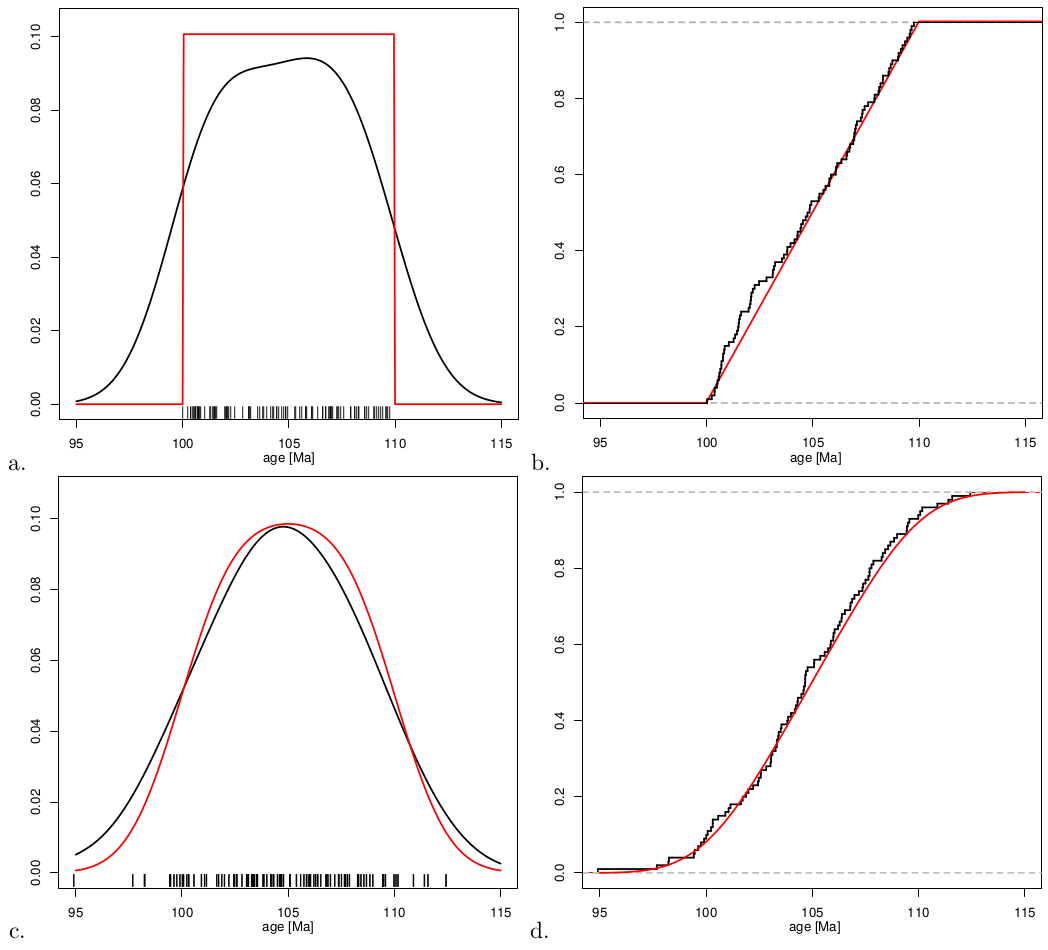
\includegraphics[width=\textwidth]{synthplots.png}
\caption{a. red -- a uniform distribution between 100 and 110 Ma,
  black -- a kernel density estimate (KDE) of 100 randomly selected
  values, which oversmooths the theoretical distribution; b. red --
  cumulative version of a., black -- Cumulative Age Distribution (CAD)
  of the 100 random samples, which does not oversmooth the theoretical
  curve; c. red -- theoretical sampling distribution in the presence
  of normally distributed analytical uncertainties ($\sigma$=1), black
  -- the KDE of 100 random samples which again oversmooth the
  theoretical curve; d. red -- the cumulative measurement
  distribution, black -- the CAD of the 100 randomly selected
  measurements is an unbiased estimator of the theoretical
  distribution.}
\label{fig:synthplots}
\end{figure}

In {\tt provenance}, CADs are obtained using an overloaded {\tt plot}
function. For example, for detrital zircon U-Pb sample {\tt N1}
(Figure \ref{fig:visualisation}a):

\begin{verbatim}
plot(DZ,snames='N1',CAD=TRUE)
\end{verbatim}

Both histograms and KDEs are implemented in standard {\tt R} as the
{\tt hist} and {\tt density} functions, respectively. These built-in
functions work very well for relatively simple, unimodal distributions
\citep{silverman1986}. However, the distributions occurring in
detrital geochronology tend to be more complex than that, causing the
{\tt density} function to overestimate the kernel bandwidth and
oversmooth the resulting distribution. For this reason, the {\tt
  provenance} package includes a separate function for kernel density
estimation using a hybrid adaptive kernel density algorithm, adopted
from {\tt DensityPlotter} \citep[version 3.0 and
  above,][]{vermeesch2012b}. This algorithm consists of two
steps. First, the fixed bandwidth algorithm by \citet{botev2010} is
used to calculate a `pilot' density.  Then, the bandwidth is adjusted
at each sample point to scale with the square root of the local
density, normalised by the geometric mean of the entire distribution
\citep{abramson1982}. Thus, the fixed bandwidth estimate is converted
into an adaptive density estimate, which assigns a narrower bandwidth
to densely sampled segments of the age distribution and a wider
bandwidth to those segments which are sparsely sampled. This increases
the resolution of the density estimates where sufficient data are
available, whilst smoothing out those parts with insufficient data. As
an example, the following code plots the U-Pb age distribution of
sample {\tt N1} from the Namibian dataset with the default settings
(Figure \ref{fig:visualisation}b):

\begin{verbatim}
N1 <- DZ$x$N1      # extract the ages of sample N1
dens <- KDE(N1)    # create the density estimate
plot(dens)         # plot the density estimate
\end{verbatim}

The appearance of the plot can be changed by modifying the optional
arguments. The following example plots the data on a logarithmic scale
from 10 to 3,000 Ma with a fixed bandwidth of 50 Ma and turns off the
sample point indicators on the x-axis (Figure \ref{fig:visualisation}c):

\begin{verbatim}
dens <- KDE(N1,bw=50,from=100,to=4000,adaptive=FALSE,log=TRUE)
plot(dens,pch=NA ) # pch = the symbol used for the sample points
\end{verbatim}

{\tt provenance} also includes some basic functionality to plot
compositional data on ternary diagrams. For example, to plot the
petrography of the Namib dataset on \citet{dickinson1983}'s QFL
diagram (Figure \ref{fig:visualisation}d):

\begin{verbatim}
plot(QFL.tern,type='QFL.dickinson')
\end{verbatim}

where {\tt QFL.tern} was produced by the {\tt ternary()} function
(Section \ref{sec:datamanipulation}). The graphical output can be
saved as a vector-editable PDF for further processing in software such
as Adobe Illustrator\copyright, CorelDraw\copyright or
Inkscape:

\begin{verbatim}
dev.copy2pdf(file="QFL.tern.pdf")
\end{verbatim}

\begin{figure}
\centering
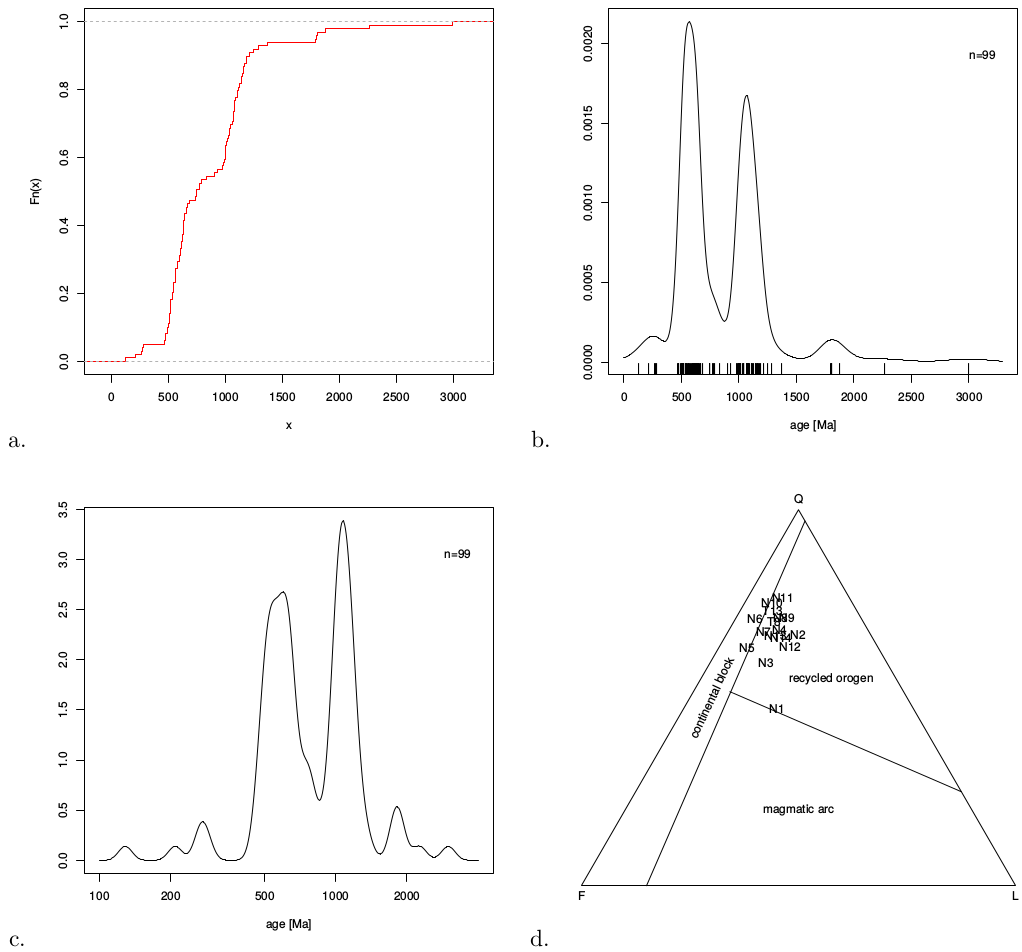
\includegraphics[width=\textwidth]{visualisation.png}
\caption{Graphical output generated by {\tt provenance} for {\tt
    distributional} and {\tt compositional} data.  a. the CAD of
  sample N1; b. the KDE of sample N1, using a the hybrid adaptive
  bandwidth algorithm outlined in Section \ref{sec:plotting}, plotted
  on a linear scale; c. a KDE using a fixed bandwidth of 50 Ma and a
  log scale; d. the quartz - feldspar - lithic composition of the
  Namib samples on \citet{dickinson1983}'s QFL diagram.}
\label{fig:visualisation}
\end{figure}

\subsection{The SRD correction: a simple way to correct 
for environmental bias}
\label{sec:srd}

To facilitate the comparison of detrital modes for provenance analysis
or stratigraphic correlation, we need to first remove the often
significant compositional differences among sediment samples that are
caused by hydrodynamic processes in the depositional
environment. Intersample modal variability can be corrected for by a
simple principle. In the absence of provenance changes and
environmental bias, the weighted average Source Rock Density (SRD) of
terrigenous grains should be equal, for each sample and each
grain-size class of each sample, to the weighted average density of
source rocks. By correcting relative abundances of detrital minerals
in proportion to their densities, we can restore the appropriate SRD
index for any provenance and subprovenance type in each sample or
grain-size class \citep{garzanti2009}. Modal variability is
effectively reduced by this procedure, which can be applied
confidently to modern sediments deposited by tractive currents in any
environment. Good results are obtained even for placer sands and
finest grain-size fractions where heavy-mineral concentration is
strongest. Such `SRD correction' also successfully compensates for
biased narrow-window modes, thus providing a numerical solution of
general validity to the problem of environmental bias in sedimentary
petrology.\\

The SRD index, used to assess average density of source rocks in the
absence of hydrodynamic effects or to detect hydraulic-controlled
concentration of denser minerals, is defined as the weighted average
density of terrigenous grains \citep[spurious and intrabasinal
  particles such as bioclasts are neglected in the
  calculation;][]{garzanti2007}:

\begin{equation}
SRD = \sum_{i=1}^n (\%m_i ~ \rho_{m_i}) = 1 / \sum_{i=1}^{n} (\%M_i / \rho_{m_i})
\label{eq:SRD}
\end{equation}

where \%m and \%M are the volume and weight percentages of mineral m,
and $\rho_m$ its density.  In order to compensate for
selective-entrainment effects, we must recalculate detrital modes for
each sample until the same SRD index is restored for each. The
mathematical procedure is similar to that used to convert volume
percentages to weight percentages, and vice-versa:

\begin{align}
\%M & = \%m ~ \rho_m / SRD = \%m ~ \rho_m / \sum_{i=1}^{n} (\%m_i ~ \rho_{m_i})  \label{eq:pctMu}\\
\%m & = \%M ~ SRD / \rho_m = \%M / \left[ \rho_m \sum_{i=1}^{n} (\%M_i / \rho_{m_i}) \right] \label{eq:pctml}
\end{align}

The `SRD correction' assumes the form of Equation \ref{eq:pctMu} for
heavy-mineral-poor samples:

\begin{equation}
\%m^* = \%m ~ \rho_m / \sum_{i=1}^{n} (\%m_i ~ \rho_{m_i})
\label{eq:SRDlight}
\end{equation}

and the form of Equation \ref{eq:pctml} for heavy-mineral-rich samples:

\begin{equation}
\%m^* = \%m / [ \rho_m \sum_{i=1}^{n} (\%m_i / \rho_{m_i}) ]
\label{eq:SRDheavy}
\end{equation}

To remove environmental bias by the SRD correction we need to assume
an appropriate common SRD value for all samples. Such a value may be
determined empirically, by averaging SRD indices of `normal' samples
with the same provenance. Or we may proceed in reverse, and find
through successive approximations the SRD value which minimizes the
residual variance in the data set. In any case, we need criteria to
tell us which SRD value is appropriate and which should be considered
anomalous.  In the absence of hydrodynamic effects, the SRD index
faithfully reflects the average density of source rocks (Garzanti et
al., 2006). With the exception of less dense glass-rich volcanic and
porous sedimentary rocks, and of denser mafic and ultramafic rocks,
rocks densities typically lie in the 2.6-2.8 g/cm$^3$ range (Daly et
al., 1966). Therefore, besides monogenic detritus supplied locally by
specific rock types (e.g., ignimbrite, gypsum, gabbro, peridotite,
granulite, eclogite), SRD indices of homogenized detritus derived
long-distance from diverse crustal sources must lie in a narrow range
(2.70 $\pm$ 0.05). Given the regional geology and geomorphology of
southern Africa, we can confidently rule out exotic compositions and
safely assume an SRD of $\sim$ 2.71. Restoring all samples from the
Namib dataset to this reference value:

\begin{verbatim}
rescomp <- restore(PTHM,dens=densities,target=2.71)
HMcomp <- c("zr","tm","rt","sph","ap","ep","gt","st","amp","cpx","opx")
PHO <- amalgamate(rescomp,Plag="P",HM=HMcomp,Opq="opaques")
plot(ternary(PHO),showpath=TRUE)
\end{verbatim}

where {\tt HMcomp} is a list of heavy minerals and {\tt amcomp}
amalgamates the restored {\tt PTHM} composition to the reference SRD
density. Setting {\tt showpath=TRUE} in the overloaded {\tt plot}
function displays the intermediate steps of the iterative SRD
correction algorithm on the ternary diagram. In the above example,
plagioclase, the amalgamated transparent heavy minerals and the opaque
minerals are plotted together because they cover a wide range of
densities (2.67, $\sim$3.5 and 5 g/cm$^3$, respectively). For the
Namib dataset, the correction path clearly shows that samples N8 and
N9 are most strongly affected by the SRD correction and, hence,
hydraulic sorting effects.  This is entirely consistent with the
interpretations of \citet{garzanti2012}, \citet{vermeesch2015}, and
Section \ref{sec:multiplemethods}. Finally, to illustrate the combined
use of {\tt provenance} with the {\tt compositions} package, the
following code adds an ellipse from the mean and the variance to the
SRD-corrected data, using the {\tt compositions} package's {\tt
  ellipses} function:

\begin{verbatim}
PHO.acomp <- as.acomp(PHO) # convert to class 'acomp'
ellipses(mean(PHO.acomp),var(PHO.acomp),r=2)
\end{verbatim}

\begin{figure}
\centering
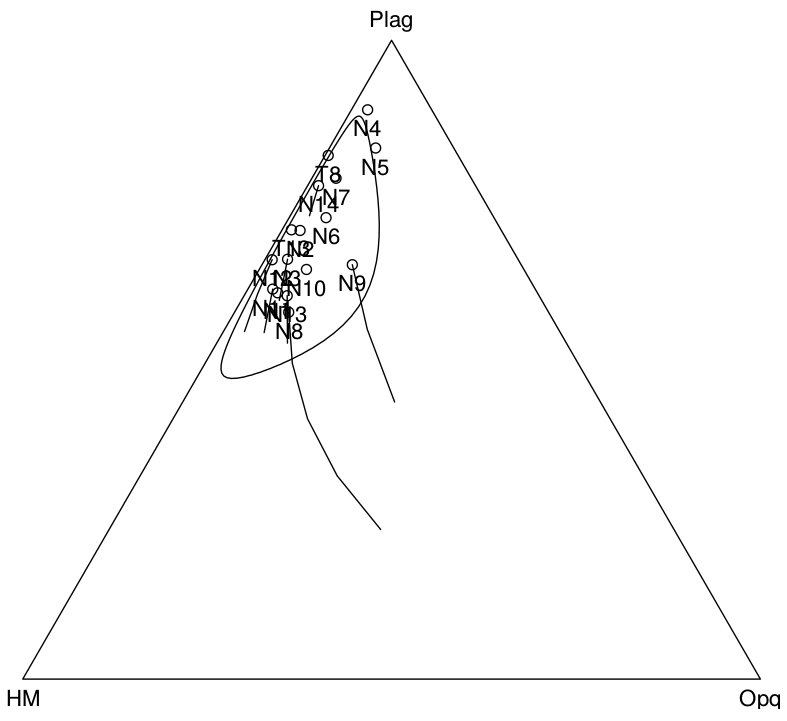
\includegraphics[width=.7\textwidth]{srd.png}
\caption{The effect of the Source Rock Density (SRD) correction on the
  Namib dataset, shown on a ternary diagram with P = plagioclase
  ($\rho$ = 2.67 g/cm$^3$), HM = heavy minerals ($\rho$ = 3.5
  g/cm$^3$), and Opq = opaque minerals ($\rho$ = 5 g/cm$^3$). Circles
  mark the restored compositions, lines connect the intermediate
  values of the SRD correction algorithm. It is evident that samples
  N8 and N9 are most strongly affected by hydraulic sorting and
  benefit from the SRD correction the most. The ellipse was drawn
  using the {\tt compositions} package's {\tt ellipses} function.}
\label{fig:srd}
\end{figure}

\subsection{Size-density sorting of detrital grains and 
intrasample variability}
\label{sec:minsorting}

The settling velocity of a detrital particle represents the balance
between gravitational forces and drag resistance due to both
turbulence and viscosity. Settling of clay and silt particles in water
is resisted by viscosity, whereas turbulence is the dominant drag
component during settling of pebbles or in air. Different empirical
formulas have been proposed to model settling of particles by tractive
currents, accounting for the wide range of grain sizes displayed by
sedimentary deposits and their diverse depositional facies (aeolian
vs. fluvial vs. marine).  The settling velocity of clay and silt
particles can be calculated by Stokes' Law:

\begin{equation}
v = g R_x D_x^2 / 18 \eta
\label{eq:stokes}
\end{equation}

where g is the gravitational constant, $R_x$ is the submerged density
($\rho_{grain}$-$\rho_{fluid}$), $D_x$ is the diameter of the
particle, and $\eta$ is the fluid viscosity.  The settling velocity of
sand-sized particles in water must be calculated by empirical
formulas, such as the relatively simple one proposed by
\citep{cheng1997}:

\begin{equation}
v = (\eta/D_x)\left[\sqrt{25 + 1.2 (g R_x D_x^3/\eta^2)^{2/3}} - 
                5\right]^{3/2}
\label{eq:cheng}
\end{equation}

The settling velocity of granules and pebbles can be described by
Newton's Impact Law:

\begin{equation}
v = \sqrt{2 g R_x D_x / (3 \rho_f)}
\label{eq:newton}
\end{equation}

where $\rho_f$ is the fluid density.  The same formula has been shown
empirically to be sufficiently accurate also to calculate the settling
of particles of any grain size in air (Garzanti et al., 2008). These
three formulas allow us to calculate the difference in nominal
diameter (the `size shift', SS) between two settling-equivalent
particles for any size, in any transporting medium, and usually
referred to quartz.  For clay and silt particles, size shifts between
any mineral x and a reference mineral or the bulk sediment are
calculated as:

\begin{equation}
SS_x = log_2(R_x/R_{ref})/2
\label{eq:SSclay}
\end{equation}

For sand sized particles: 

\begin{equation}
SS_x = log_2(R_x/R_{ref}) - (3/2) log_2 (\Xi_m/\Xi_{ref})
\label{eq:SSsand}
\end{equation}

where $\Xi = v/\eta + \sqrt{(v/\eta)^2 + 48 (g ~
  R_x/\eta^2)^{2/3}}$. For granules and pebbles or any sediment
settling in air, size shifts are twice those predicted by Stokes' Law:

\begin{equation}
SS_x = log_2(R_x/R_{ref})
\label{eq:SSgravel}
\end{equation}

The average settling velocity for each given sediment sample can be
calculated with formulas \ref{eq:stokes}, \ref{eq:cheng} or
\ref{eq:newton} according to its mean grain size, grain density (SRD
index of the bulk sediment, see Section \ref{sec:srd}) and
depositional environment (air, freshwater or seawater). For each
detrital mineral or rock fragment, the size shift referred to the
bulk-sediment (SRD index) is calculated with formulas \ref{eq:SSclay},
\ref{eq:SSsand} or \ref{eq:SSgravel}. To account for shape effects
\citep{komar1984}, the density of micas is lowered by 0.5 g/cm$^3$
\citep{garzanti2008}. Finally, a Gaussian size-frequency distribution
is calculated for each detrital component by combining its size shift
referred to the mean size of the bulk sediment and the sorting value
of the latter.\\

In {\tt provenance}, all these calculations are performed by the
{\tt minsorting} function, so named after the spreadsheet application
of \citet{resentini2013} on which it is based. To illustrate the use
of the {\tt minsorting} function, the following code snippet applies
it to one of the end-member compositions included with the package,
assuming a mean grain size of (Krumbein) $\Phi$=2 and standard
deviation $\Phi$=1:

\begin{verbatim}
data(endmembers,densities)
distribution <- minsorting(endmembers,densities,sname='ophiolite',
                           phi=2,sigmaphi=1,medium="seawater",by=0.05)
plot(distribution,components=c('F','px','opaques'))
\end{verbatim}

Which yields the grain size distribution of feldspar, pyroxene and
opaque minerals (in 0.05 $\Phi$ intervals), so chosen because of the
great contrast in density between them (Figure \ref{fig:minsorting}).
When - as is commonly done in geochronological analysis - one specific
mineral is targeted (e.g., apatite or zircon), we can use such
information to choose the most suitable size window for laboratory
treatment and analysis, and thus obtain a most faithful
characterization of the sediment sample.

\begin{figure}
\centering
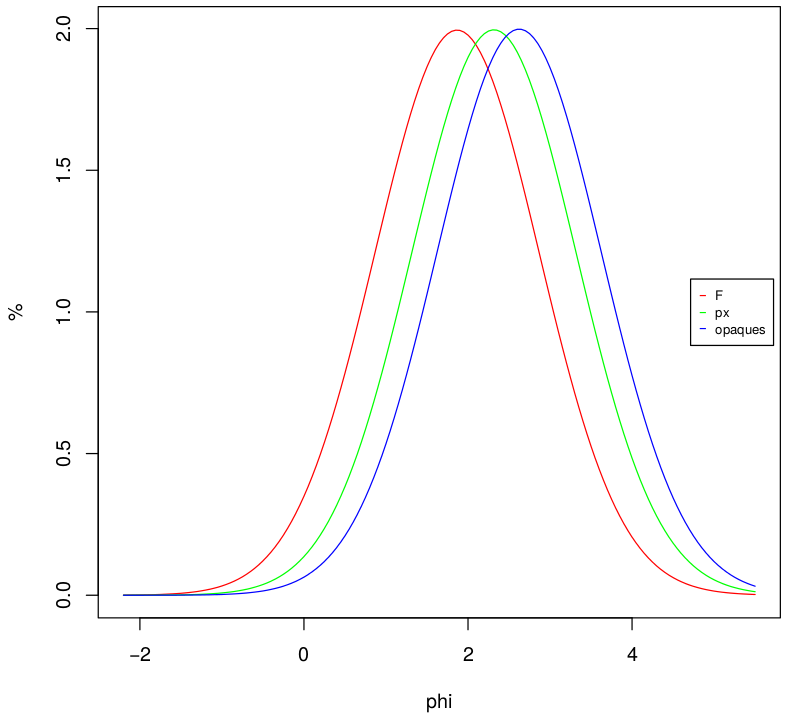
\includegraphics[width=.7\textwidth]{minsorting.png}
\caption{Graphical output of the {\tt minsorting} routine applied to
  an ophiolitic end-member composition. Different colours show the
  inferred grain-size distribution of feldspars (`F', red), pyroxene
  (`px', blue) and opaque minerals (green) in Krumbein's $\Phi$ units,
  assuming a mean grain size for the bulk sediment of $\Phi$=2 with
  standard deviation $\Phi$=1.  It can be seen that relatively coarse
  grains of the comparatively light minerals are hydraulically
  equivalent with finer grains of the dense minerals.}
\label{fig:minsorting}
\end{figure}

\section{Jointly considering multiple samples}
\label{sec:multiplesamples}

{\tt provenance} allows multiple samples to be plotted together. For
example, to plot all 16 detrital age distributions from the Namibian
dataset on a scale from 0 to 3,000 Ma in four columns:

\begin{verbatim}
UPb <- KDEs(DZ,from=0,to=3000,normalise=TRUE)
summaryplot(UPb,ncol=4)
\end{verbatim}

where the {\tt normalise} flag sets the area under each of the KDEs
to the same value. The resulting plot contains 16 kernel density
estimates, resulting in 16 $\times$ 15 / 2 = 120 pairwise comparisons
(Figure \ref{fig:KDEs}). The first step towards simplifying this
multi-sample comparison problem is to convert the raw data into a
table of pairwise distances. This can be achieved using a number of
different dissimilarity measures.

\begin{figure}
\centering
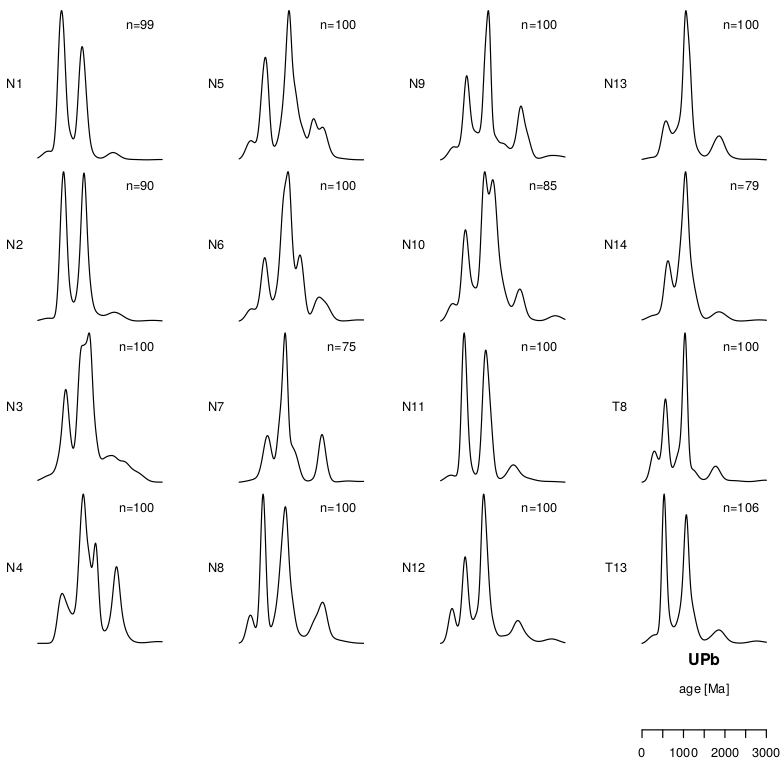
\includegraphics[width=.7\textwidth]{KDEs.png}
\caption{Graphical output of the {\tt summaryplot} function, applied
  to the detrital zircon U-Pb age data. The areas under the KDEs have
  been normalised to the same value.}
\label{fig:KDEs}
\end{figure}

\subsection{Dissimilarity measures}
\label{sec:dissimilarity}

A crucial first step towards simplifying the interpretation of
multi-sample datasets is to replace the visual comparison of age
distributions, histograms and pie charts with numerical values
expressing the `dissimilarity' between samples. For distributional
data, the default method is the Kolmogorov-Smirnov (K-S) statistic
($\delta^{ks}_{AB}$), which uses the maximum absolute difference
between two cumulative distributions \citep{feller1948}. Given two
samples A and B, the K-S distance is defined as

\begin{equation}
\delta^{ks}_{AB} = \underset{t}{max}|F_A(t)-F_B(t)|
\label{eq:ks}
\end{equation}

where F$_A$ and F$_B$ are defined by Equation \ref{eq:cdf} and
$|\cdot|$ stands for the absolute value.  One nice feature of the K-S
distance is that it obeys the triangle inequality, which states that,
for any three samples A, B and C, the distance between A and C is less
than or equal to the distance between A and B plus the distance
between B and C. The triangle inequality makes the K-S distance behave
like the physical distances which we are familiar with in the real
world.  On the other hand, the K-S statistic also has limitations,
such as its inability to take into account the effect of unequal
analytical uncertainties. This makes it difficult to objectively
compare samples acquired on different mass spectrometers characterised
by differing analytical precision. This problem was addressed by
\citet{sircombe2004a} using the squared overlap between so-called
Kernel Functional Estimates (KFEs):

\begin{equation}
\delta^{sh}_{AB} = \sqrt{\int\left(f_A(t)-f_B(t)\right)^2dt}
\label{eq:sh}
\end{equation}

where $f_A$ and $f_B$ are the KFEs of samples A and B. KFEs are a
special type of KDEs, in which a variable degree of deliberate
oversmoothing is applied to the different samples to account for the
differing analytical uncertainties between them
\citep{sircombe2004a}. Although KFEs are useful as a point of
comparison between different samples, they have limited value as a
data visualisation tool due to the oversmoothing. To use the S-H
dissimilarity, the user needs to supply the analytical uncertainties
in a separate {\tt .csv} file. The following code demonstrates the
calculation of K-S and S-H dissimilarities in {\tt provenance}:

\begin{verbatim}
KS.diss <- diss(DZ,method='KS')
SH.diss <- diss(DZ,method='SH')
\end{verbatim}

For compositional proxies such as petrographic, heavy mineral or
chemical data, {\tt provenance} provides a further two dissimilarity
measures. If the dataset is free of zero values, Aitchison's central
logratio distance is used by default:

\begin{equation}
\delta^{ait}_{AB} = \sqrt{\sum\limits_{i=1}^{n} \left[
ln\left(\frac{A_i}{g(A)}\right) - ln\left(\frac{B_i}{g(B)}\right)
\right]^2}
\label{eq:aitchison}
\end{equation}

where `g(x)’ stands for `the geometric mean of x’
\citep{aitchison1986, vermeesch2013}.  Note that the same distance is
obtained irrespective of whether the input data are expressed as
fractions or percentages. The Aitchison distance breaks down for
datasets comprising `zero counts' ($A_i$ = 0 or $B_i$=0 for any $i$).
This problem can be solved by pooling several categories together (see
Section \ref{sec:datamanipulation}), or by using a different
dissimilarity measure such as the Bray-Curtis distance:

\begin{equation}
\delta^{bc}_{AB} = \sum\limits_{i=1}^{n} |A_i - B_i| \Big/ 
                 \sum\limits_{i=1}^{n} (A_i + B_i)
\label{eq:bray}
\end{equation}

The following example yields the dissimilarity matrices of the heavy
mineral and major element compositions using the Bray-Curtis and
Aitchison measures, respectively:

\begin{verbatim}
HM.diss <- diss(HM,method='bray')
Major.diss <- diss(Major,method='aitchison')
\end{verbatim}

\subsection{Principal Component Analysis and Multidimensional Scaling}
\label{sec:PCAMDS}

Although the dissimilarity matrices introduced in the previous section
make the comparison of two samples more objective, it remains
difficult to discern any meaningful patterns in large numbers of such
pairwise comparisons. Multidimensional Scaling (MDS) is a
dimension-reducing technique which can make the comparison of multiple
samples more objective \citep{borg2005}. MDS is widely used in other
scientific disciplines and can easily be adapted for provenance
studies \citep{vermeesch2013}. Given a table of pairwise distances
between samples, MDS produces a configuration of points in which
similar samples plot close together and dissimilar samples plot far
apart. {\tt provenance} implements both {\it classical} MDS, in which
the physical distances between the different points in the MDS
configuration are directly proportional to the dissimilarities between
the corresponding samples; and {\it nonmetric} MDS, which merely aims
to reproduce the relative ranks of the dissimilarities
\citep{borg2005}. In the latter case, {provenance} allows the user to
graphically assess the goodness of fit by plotting the dissimilarities
against the fitted distances on a so-called `Shepard Plot'
\citep{kruskal1978}. {\tt provenance} uses nonmetric MDS by default
because it produces better fits than classical MDS and accepts a wider
range of dissimilarity measures \citep{kruskal1978, borg2005}. The
{\tt MDS} function accepts as input either data of class {\tt
  compositional} or {\tt distributional}, or a dissimilary matrix
(class {\tt diss}).  The following two lines of code are therefore
equivalent to each other:

\begin{verbatim}
MDS.DZ.1 <- MDS(DZ)
MDS.DZ.2 <- MDS(diss(DZ))
\end{verbatim}

In contrast with nonmetric MDS, classical MDS can only be used for
dissimilarity measures are proper distances and therefore fulfil the
triangle inequality \citep{borg2005}, which is the case for the
Kolmogorov-Smirnov and Aitchison distances. For example, using the
latter dissimilarity measure, the major element composition can be
plotted as a classical MDS configuration:

\begin{verbatim}
Major.diss <- diss(Major,method='aitchison')
MDS.Major <- MDS(Major.diss,classical=TRUE)
plot(MDS.Major,xaxt='s',yaxt='s')
\end{verbatim}

Where the {\tt xaxt} and {\tt yaxt} flags add tick marks and labels to
the x and y axes (these are turned off by default). By definition, the
Aitchison distance does not only fulfil the triangle inequality but is
a Euclidean distance as well. In this case, MDS is equivalent to
Principal Component Analysis \citep[PCA,][]{aitchison1983, cox2000}.
This equivalence can be demonstrated by the fact that:

\begin{verbatim}
PCA.Major <- PCA(Major)
plot(PCA.Major)
\end{verbatim}

produces identical output as the previous code snippet (Figure
\ref{fig:MDSPCA}). The main advantage of PCA over MDS is that it can
be visualised as a `biplot', in which the configuration is accompanied
by a set of vector `loadings' showing the relationship between the
categorical input variables (Figure \ref{fig:MDSPCA}.b). Thus, the PCA
biplot facilitates the interpretation of the configuration in terms of
underlying processes \citep{aitchison2002}.  In this respect,
compositional biplots are similar to a 3-way extension of the MDS
method called INDSCAL, which is discussed in the next section. One
limitation of compositional PCA is its inability to handle datasets
containing zero values, which is due to its dependence on logratios
(see Section \ref{sec:dissimilarity}). Various ways have been proposed
to deal with this problem \citep[e.g.,][]{martin2003}, but none of
these are implemented in {\tt provenance} (yet).  Instead, the user is
presented with two options. The zero-value problem can either be
circumvented by employing non-metric MDS using the Bray-Curtis
dissimilarity; or by resorting to the PCA functionality implemented in
the {\tt compositions} and {\tt robCompositions} packages.

\begin{figure}
\centering
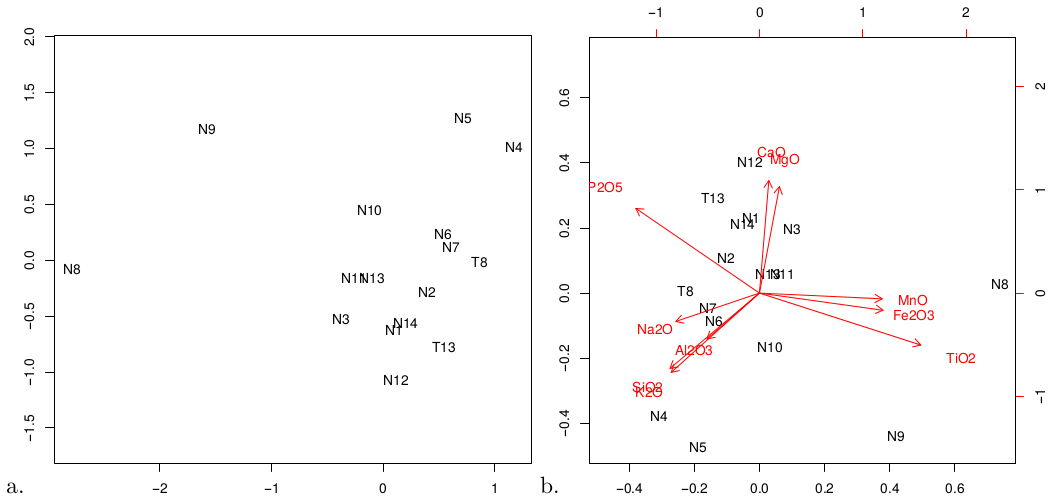
\includegraphics[width=.46\textwidth]{MDSPCA.png}
\caption{Illustration of the equivalence of Multidimensional Scaling
  (MDS, a) and Principal Component Analysis (PCA, b) for compositional
  data using the Aitchison dissimilarity, using the major element
  composition of the Namib samples as an example. The two
  configurations are identical apart from an arbitrary rotation.}
\label{fig:MDSPCA}
\end{figure}

\section{Combining multiple methods in multiple samples}
\label{sec:multiplemethods}

The entire 5-proxy dataset can be visualised together with the {\tt
  summaryplot} command, producing a diagram with 16 KDEs and 64 pie
charts:

\begin{verbatim}
PT$colmap <- 'cm.colors'
Trace$colmap <- 'rainbow'
UPb <- KDEs(DZ,from=0,to=3000,normalise=TRUE)
summaryplot(UPb,HM,PT,Major,Trace,ncol=2)
\end{verbatim}

Which assigns a different colour map to the pie charts of the
petrographic and trace element data from the default {\tt
  heat.colors}. The summary plot manages to squeeze 16,125 numerical
values into a single diagram, which provides a good visual
illustration of the term `Big Data', but is next to impossible to
interpret geologically. Using the methods introduced in Section
\ref{sec:multiplesamples}, we can produce five MDS maps and thereby
facilitate the multi-sample comparison for each dataset
\citep{vermeesch2015}. Unfortunately, the subtle differences between
these maps present a second type of multiple comparison problem, which
calls for second layer of statistical simplification.  The {\tt
  provenance} package provides two alternative solutions for this:
Procrustes analysis and 3-way MDS.\\

Procrustes analysis is the process by which a combination of
shape-preserving transformations is used to match the shape of one
object with that of another. Generalised Procrustes Analysis (GPA) is
a generalisation of this procedure to multiple objects. In a
provenance context, GPA extracts a single `consensus' view from a
collection of MDS configurations, by rotating, reflecting and scaling
them to minimise a least squares criterion \citep{gower1975,
  vermeesch2015}. The following code applies this method to the Namib
dataset:

\begin{verbatim}
proc <- procrustes(DZ,HM,PT,Major,Trace)
plot(proc)
\end{verbatim}

GPA is a two step process, in which the individual datasets are first
subjected to an MDS analysis, and the resulting configurations are
then transformed into a group configuration. Alternatively, the same
type of graphical output can be generated in a single step, using the
final technique discussed in this paper, 3-way MDS.\\

As the name suggests, 3-way MDS is a generalisation of the methods
discussed in Section \ref{sec:PCAMDS} from two- to three-dimensional
dissimilarity matrices.  For the Namib dataset, the combination of 16
samples and 5 methods results in a dissimilarity matrix of size 15
$\times$ 15 $\times$ 5. There exist many types of 3-way MDS
algorithms, the oldest and most widely used of which is called
INdividual Differences SCALing \citep[INDSCAL,][]{carroll1970}. In
contrast with 2-way MDS and GPA, INDSCAL produces not one but two
pieces of graphical output: the `group configuration' and the `source
weights'. For the Namib dataset, the former reproduces the relative
dissimilarities between the samples, whereas the latter displays the
relationship between the provenance proxies
\citep{vermeesch2015}. This is similar in a way to the compositional
biplots produced by PCA (Section \ref{sec:PCAMDS}), which
simultaneously display the configuration of the samples and the
relationship between the variables (e.g. minerals or chemical
elements).  In the case of INDSCAL, the `source weights' quantify the
relative importance attached by each of the data sources
(i.e. provenance proxies) to the horizontal and vertical axis of the
`group configuration' \citep{carroll1970, deleeuw2011, vermeesch2015}.
In {\tt provenance}:

\begin{verbatim}
IND <- indscal(DZ,HM,PT,Trace,Major)
plot(IND) 
\end{verbatim}

Note that the resulting group configuration (Figure
\ref{fig:indscal}.a) looks significantly different from that presented
by \citet{vermeesch2015}. This is due to an error in the original
petrographic data table, which has been fixed in the present
paper. The `source' weights (Figure \ref{fig:indscal}.b) show that the
major and trace element compositions attach much greater weight to the
horizontal axis of the group configuration than the other
proxies. This is attributed to hydraulic sorting, which affects bulk
compositions more than it does mineral separates
\citep{vermeesch2015}. This is entirely consistent with Figure
\ref{fig:srd}, which showed that samples N8 and N9 are particularly
affected by winnowing effects.

\begin{figure}
\centering
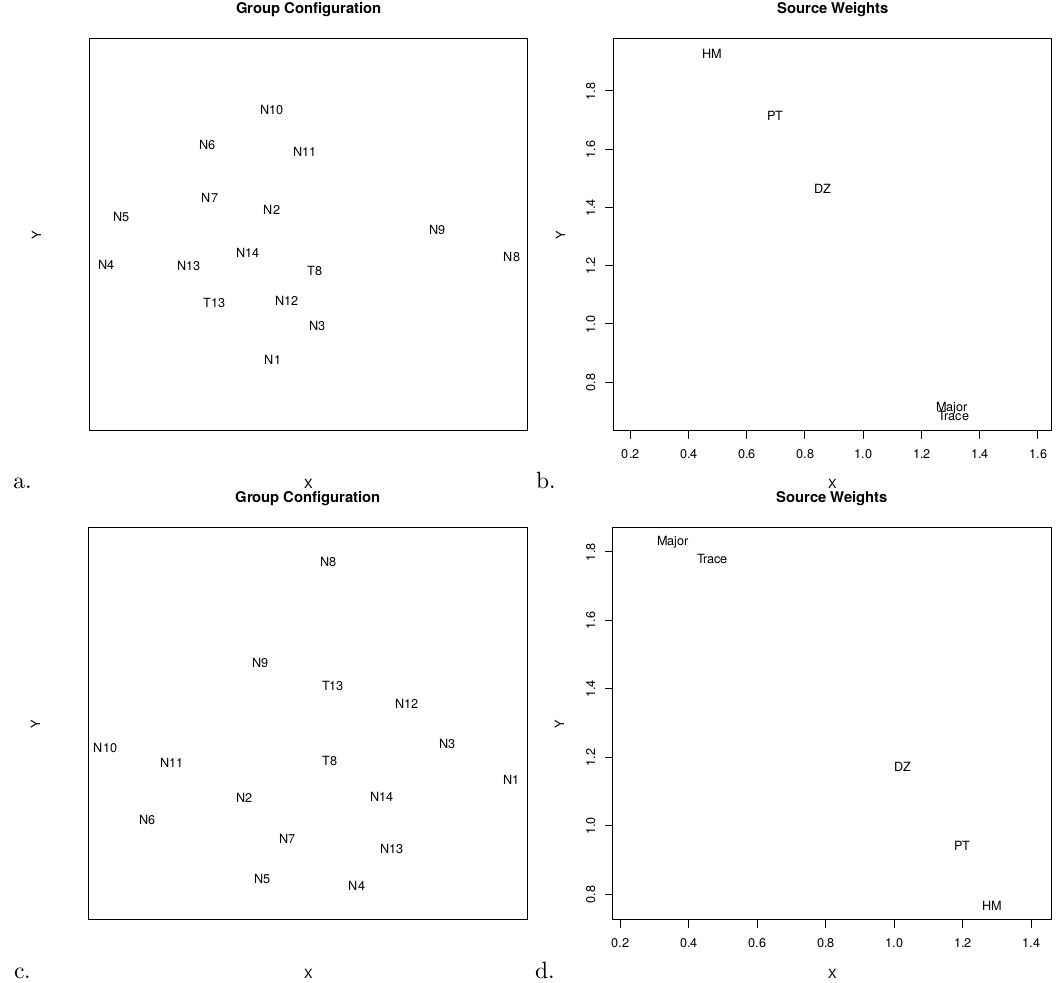
\includegraphics[width=\textwidth]{indscal.png}
\caption{a. group configuration of an INDSCAL analysis of the Namib
  dataset using the Kolmogorov-Smirnov dissimilarity for the U-Pb data
  (DZ), the Bray-Curtis dissimilarity for the heavy mineral (HM) and
  bulk petrography (PT) data, and the Aitchison distance for the major
  and trace element compositions; b. the source weights, which show
  the relative importance which each of the five provenance proxies
  attach to the horizontal and vertical axis of the group
  configuration \citep{vermeesch2015}; note that samples N8 and N9
  plot on the far right of the group configuration, indicating that
  they have significantly different Major and Trace element
  compositions. This is consistent with these samples being affected
  by hydraulic sorting, as was previously shown in Figure
  \ref{fig:srd}. c. the group configuration of the same data, but
  using the Sircombe-Hazelton dissimilarity for the U-Pb data, and the
  Bray-Curtis dissimilarity for the major and trace compositions;
  d. the correponding source weights. Although the two configurations
  look very similar, the actual weights attached to each of the
  proxies are very different.}
\label{fig:indscal}
\end{figure}

Although, in principle, 3-way MDS yields more insightful output than
GPA, in practice things do not always work out so well. The problem is
that the output of INDSCAL is often very sensitive to subtle changes
in the input data.  For example, running INDSCAL on the same data as
before, but using the S-H dissimilarity instead of the K-S distance
for the DZ data and the Bray-Curtis distance instead of the Aitchison
distance for the bulk chemistry results in a similar looking group
configurations (Figure \ref{fig:indscal}.c), but a significantly
different subject weights (Figure \ref{fig:indscal}.d).

\begin{verbatim}
DZ$method <- "SH"
Major$method <- "bray"
Trace$method <- "bray"
IND.SH <- indscal(DZ,HM,PT,Trace,Major)
plot(IND.SH) 
\end{verbatim}

It is therefore advisable not to overinterpret these weights, and thus
in practice INDSCAL often does not outperform GPA as might be hoped.

\section{Conclusions}
\label{sec:conclusions}

It is increasingly being recognised that, in order to truly understand
sediment routing systems, the combination of multiple proxies teaches
more than the sum of its parts \citep{garzanti2015}.  This paper
introduced an {\tt R} package named {\tt provenance} to facilitate the
joint interpretation of large datasets comprising many samples and
several provenance proxies. Technological advances such as fast
scanning electron microscopes \citep[e.g, QEMSCAN,][]{allen2012} and
high-throughput LA-ICP-MS \citep[e.g.,][]{frei2009} promise to fully
unlock the power of multi-method provenance analysis and further
increase the need for the `Big Data' analysis tools provided by {\tt
  provenance}.  Much work remains to be done to extend the methods
presented in this paper.  One example is the incorporation of
dissimilarity measures to compare distributional data of higher
dimensionality, such as paired U-Pb ages and Hf- or O-isotopic
compositions \citep[e.g.,][]{owen1987}.  Another example is the
introduction of weighted MDS \citep{deleeuw2009} to handle, say,
datasets containing samples of widely different sizes.\\

We would like to conclude this paper with the advice not to rely
exclusively on statistics for the interpretation of provenance
data. It is our opinion that statistical provenance analysis should be
used as a complement to rather than a substitute for expert geological
knowledge.  It is sometimes found that petrographic information,
especially the composition of the lithic fragments, allows an
experienced analyst to unequivocally constrain provenance with much
greater confidence than any machine or computer algorithm
\citep{garzanti2015}. Like any `black box' technique, statistical
methods such as MDS or INDSCAL can easily be abused.  By exhaustively
going through all the options provided by {\tt provenance}, it may be
possible to `cherry pick' a configuration that supports a
pre-conceived model.  Paraphrasing Andrew Lang, we would like to urge
the user to resist the temptation of using {\tt provenance} in the
same way that a drunk uses lamp-posts -- for support rather than
illumination.  It is important to keep in mind that good scientific
practice involves testing and rejecting rather than `proving'
hypotheses \citep{popper1959}.  We hope that {\tt provenance} will be
used according to this philosophy, along with all the other techniques
at the disposal of sedimentary geologist today.

\section*{Acknowledgments}

The author would like to thank Istv\'{a}n Dunkl, Luca Caracciolo,
Hilmar von Eynatten and Guido Meinhold for organising the 2014 Working
Group for Sediment Generation workshop in G\"{o}ttingen and inviting
him to present the work behind the {\tt provenance} package.  This
research was funded by NERC standard grant \#NE/1009248/1 and ERC
starting grant 259505 (`KArSD'). Raimon Tolosana-Delgado and two
anonymous reviewers are gratefully acknowledged for their critical but
constructive comments which truly transformed the paper.

%\bibliographystyle{elsarticle-harv}
%\bibliography{/home/pvermees/Dropbox/biblio}

\begin{thebibliography}{48}
\expandafter\ifx\csname natexlab\endcsname\relax\def\natexlab#1{#1}\fi
\providecommand{\url}[1]{\texttt{#1}}
\providecommand{\href}[2]{#2}
\providecommand{\path}[1]{#1}
\providecommand{\DOIprefix}{doi:}
\providecommand{\ArXivprefix}{arXiv:}
\providecommand{\URLprefix}{URL: }
\providecommand{\Pubmedprefix}{pmid:}
\providecommand{\doi}[1]{\href{http://dx.doi.org/#1}{\path{#1}}}
\providecommand{\Pubmed}[1]{\href{pmid:#1}{\path{#1}}}
\providecommand{\bibinfo}[2]{#2}
\ifx\xfnm\relax \def\xfnm[#1]{\unskip,\space#1}\fi
%Type = Article
\bibitem[{Abramson(1982)}]{abramson1982}
\bibinfo{author}{Abramson, I.S.}, \bibinfo{year}{1982}.
\newblock \bibinfo{title}{On bandwidth variation in kernel estimates-a square
  root law}.
\newblock \bibinfo{journal}{The Annals of Statistics} ,
  \bibinfo{pages}{1217--1223}.
%Type = Article
\bibitem[{Aitchison(1983)}]{aitchison1983}
\bibinfo{author}{Aitchison, J.}, \bibinfo{year}{1983}.
\newblock \bibinfo{title}{Principal component analysis of compositional data}.
\newblock \bibinfo{journal}{Biometrika} \bibinfo{volume}{70},
  \bibinfo{pages}{57--65}.
\newblock \DOIprefix\doi{10.1093/biomet/70.1.57}.
%Type = Book
\bibitem[{Aitchison(1986)}]{aitchison1986}
\bibinfo{author}{Aitchison, J.}, \bibinfo{year}{1986}.
\newblock \bibinfo{title}{The statistical analysis of compositional data}.
\newblock \bibinfo{publisher}{London, Chapman and Hall}.
%Type = Article
\bibitem[{Aitchison and Greenacre(2002)}]{aitchison2002}
\bibinfo{author}{Aitchison, J.}, \bibinfo{author}{Greenacre, M.},
  \bibinfo{year}{2002}.
\newblock \bibinfo{title}{Biplots of compositional data}.
\newblock \bibinfo{journal}{Journal of the Royal Statistical Society: Series C
  (Applied Statistics)} \bibinfo{volume}{51}, \bibinfo{pages}{375--392}.
%Type = Article
\bibitem[{Allen et~al.(2012)Allen, Johnson, Heumann, Gooley and
  Gallin}]{allen2012}
\bibinfo{author}{Allen, J.L.}, \bibinfo{author}{Johnson, C.L.},
  \bibinfo{author}{Heumann, M.J.}, \bibinfo{author}{Gooley, J.},
  \bibinfo{author}{Gallin, W.}, \bibinfo{year}{2012}.
\newblock \bibinfo{title}{{New technology and methodology for assessing
  sandstone composition: A preliminary case study using a quantitative electron
  microscope scanner (QEMScan)}}.
\newblock \bibinfo{journal}{Geological Society of America Special Papers}
  \bibinfo{volume}{487}, \bibinfo{pages}{177--194}.
%Type = Article
\bibitem[{Avdeev et~al.(2011)Avdeev, Niemi and Clark}]{avdeev2011}
\bibinfo{author}{Avdeev, B.}, \bibinfo{author}{Niemi, N.A.},
  \bibinfo{author}{Clark, M.K.}, \bibinfo{year}{2011}.
\newblock \bibinfo{title}{Doing more with less: Bayesian estimation of erosion
  models with detrital thermochronometric data}.
\newblock \bibinfo{journal}{Earth and Planetary Science Letters}
  \bibinfo{volume}{305}, \bibinfo{pages}{385--395}.
%Type = Article
\bibitem[{Basu and Molinaroli(1989)}]{basu1989}
\bibinfo{author}{Basu, A.}, \bibinfo{author}{Molinaroli, E.},
  \bibinfo{year}{1989}.
\newblock \bibinfo{title}{{Provenance characteristics of detrital opaque Fe-Ti
  oxide minerals}}.
\newblock \bibinfo{journal}{Journal of Sedimentary Research}
  \bibinfo{volume}{59}.
%Type = Article
\bibitem[{van~den Boogaart and Tolosana-Delgado(2008)}]{vandenboogaart2008}
\bibinfo{author}{van~den Boogaart, K.G.}, \bibinfo{author}{Tolosana-Delgado,
  R.}, \bibinfo{year}{2008}.
\newblock \bibinfo{title}{"{C}ompositions": a unified {R} package to analyze
  compositional data}.
\newblock \bibinfo{journal}{Computers \& Geosciences} \bibinfo{volume}{34},
  \bibinfo{pages}{320--338}.
%Type = Book
\bibitem[{Borg and Groenen(2005)}]{borg2005}
\bibinfo{author}{Borg, I.}, \bibinfo{author}{Groenen, P.J.},
  \bibinfo{year}{2005}.
\newblock \bibinfo{title}{Modern multidimensional scaling: Theory and
  applications}.
\newblock \bibinfo{publisher}{Springer}.
%Type = Article
\bibitem[{{Botev} et~al.(2010){Botev}, {Grotowski} and {Kroese}}]{botev2010}
\bibinfo{author}{{Botev}, Z.I.}, \bibinfo{author}{{Grotowski}, J.F.},
  \bibinfo{author}{{Kroese}, D.P.}, \bibinfo{year}{2010}.
\newblock \bibinfo{title}{{Kernel density estimation via diffusion}}.
\newblock \bibinfo{journal}{Annals of Statistics} \bibinfo{volume}{38},
  \bibinfo{pages}{2916--2957}.
%Type = Article
\bibitem[{Carroll and Chang(1970)}]{carroll1970}
\bibinfo{author}{Carroll, J.D.}, \bibinfo{author}{Chang, J.J.},
  \bibinfo{year}{1970}.
\newblock \bibinfo{title}{{Analysis of individual differences in
  multidimensional scaling via an N-way generalization of “Eckart-Young”
  decomposition}}.
\newblock \bibinfo{journal}{Psychometrika} \bibinfo{volume}{35},
  \bibinfo{pages}{283--319}.
%Type = Article
\bibitem[{Cheng(1997)}]{cheng1997}
\bibinfo{author}{Cheng, N.S.}, \bibinfo{year}{1997}.
\newblock \bibinfo{title}{Simplified settling velocity formula for sediment
  particle}.
\newblock \bibinfo{journal}{Journal of hydraulic engineering}
  \bibinfo{volume}{123}, \bibinfo{pages}{149--152}.
%Type = Book
\bibitem[{Cox and Cox(2000)}]{cox2000}
\bibinfo{author}{Cox, T.F.}, \bibinfo{author}{Cox, M.A.}, \bibinfo{year}{2000}.
\newblock \bibinfo{title}{Multidimensional scaling}.
\newblock \bibinfo{publisher}{CRC Press}.
%Type = Article
\bibitem[{De~Leeuw and Mair(2011)}]{deleeuw2011}
\bibinfo{author}{De~Leeuw, J.}, \bibinfo{author}{Mair, P.},
  \bibinfo{year}{2011}.
\newblock \bibinfo{title}{{Multidimensional scaling using majorization: SMACOF
  in R}}.
\newblock \bibinfo{journal}{Department of Statistics, UCLA} .
%Type = Article
\bibitem[{Dickinson et~al.(1983)Dickinson, Beard, Brakenridge, Erjavec,
  Ferguson, Inman, Knepp, Lindberg and Ryberg}]{dickinson1983}
\bibinfo{author}{Dickinson, W.R.}, \bibinfo{author}{Beard, L.S.},
  \bibinfo{author}{Brakenridge, G.R.}, \bibinfo{author}{Erjavec, J.L.},
  \bibinfo{author}{Ferguson, R.C.}, \bibinfo{author}{Inman, K.F.},
  \bibinfo{author}{Knepp, R.A.}, \bibinfo{author}{Lindberg, F.A.},
  \bibinfo{author}{Ryberg, P.T.}, \bibinfo{year}{1983}.
\newblock \bibinfo{title}{{Provenance of North American Phanerozoic sandstones
  in relation to tectonic setting}}.
\newblock \bibinfo{journal}{Geological Society of America Bulletin}
  \bibinfo{volume}{94}, \bibinfo{pages}{222--235}.
%Type = Article
\bibitem[{Dodson et~al.(1988)Dodson, Compston, Williams and
  Wilson}]{dodson1988}
\bibinfo{author}{Dodson, M.}, \bibinfo{author}{Compston, W.},
  \bibinfo{author}{Williams, I.}, \bibinfo{author}{Wilson, J.},
  \bibinfo{year}{1988}.
\newblock \bibinfo{title}{{A search for ancient detrital zircons in Zimbabwean
  sediments}}.
\newblock \bibinfo{journal}{Journal of the Geological Society}
  \bibinfo{volume}{145}, \bibinfo{pages}{977--983}.
\newblock \DOIprefix\doi{10.1144/​gsjgs.145.6.0977}.
%Type = Article
\bibitem[{Feller(1948)}]{feller1948}
\bibinfo{author}{Feller, W.}, \bibinfo{year}{1948}.
\newblock \bibinfo{title}{On the {K}olmogorov-{S}mirnov limit theorems for
  empirical distributions}.
\newblock \bibinfo{journal}{The Annals of Mathematical Statistics}
  \bibinfo{volume}{19}, \bibinfo{pages}{177--189}.
%Type = Article
\bibitem[{Frei and Gerdes(2009)}]{frei2009}
\bibinfo{author}{Frei, D.}, \bibinfo{author}{Gerdes, A.}, \bibinfo{year}{2009}.
\newblock \bibinfo{title}{{Precise and accurate {\it in situ} U--Pb dating of
  zircon with high sample throughput by automated LA-SF-ICP-MS}}.
\newblock \bibinfo{journal}{Chemical Geology} \bibinfo{volume}{261},
  \bibinfo{pages}{261--270}.
%Type = Article
\bibitem[{Garzanti(2015)}]{garzanti2015}
\bibinfo{author}{Garzanti, E.}, \bibinfo{year}{2015}.
\newblock \bibinfo{title}{From static to dynamic provenance analysis -
  sedimentary petrology upgraded}.
\newblock \bibinfo{journal}{Sedimentary Geology} \bibinfo{volume}{(this
  issue)}.
%Type = Incollection
\bibitem[{Garzanti and And{\`{o}}(2007)}]{garzanti2007}
\bibinfo{author}{Garzanti, E.}, \bibinfo{author}{And{\`{o}}, S.},
  \bibinfo{year}{2007}.
\newblock \bibinfo{title}{Heavy-mineral concentration in modern sands:
  implications for provenance interpretation}, in: \bibinfo{editor}{Mange, M.},
  \bibinfo{editor}{Wright, D.} (Eds.), \bibinfo{booktitle}{Heavy Minerals in
  Use, {D}evelopments in {S}edimentology {S}eries 58}.
  \bibinfo{publisher}{Elsevier, Amsterdam}, pp. \bibinfo{pages}{517--545}.
%Type = Article
\bibitem[{Garzanti et~al.(2008)Garzanti, And{\`o} and Vezzoli}]{garzanti2008}
\bibinfo{author}{Garzanti, E.}, \bibinfo{author}{And{\`o}, S.},
  \bibinfo{author}{Vezzoli, G.}, \bibinfo{year}{2008}.
\newblock \bibinfo{title}{Settling equivalence of detrital minerals and
  grain-size dependence of sediment composition}.
\newblock \bibinfo{journal}{Earth and Planetary Science Letters}
  \bibinfo{volume}{273}, \bibinfo{pages}{138--151}.
%Type = Article
\bibitem[{{Garzanti} et~al.(2009){Garzanti}, {And{\`o}} and
  {Vezzoli}}]{garzanti2009}
\bibinfo{author}{{Garzanti}, E.}, \bibinfo{author}{{And{\`o}}, S.},
  \bibinfo{author}{{Vezzoli}, G.}, \bibinfo{year}{2009}.
\newblock \bibinfo{title}{{Grain-size dependence of sediment composition and
  environmental bias in provenance studies}}.
\newblock \bibinfo{journal}{Earth and Planetary Science Letters}
  \bibinfo{volume}{277}, \bibinfo{pages}{422--432}.
\newblock \DOIprefix\doi{10.1016/j.epsl.2008.11.007}.
%Type = Article
\bibitem[{Garzanti et~al.(2012)Garzanti, And{\`o}, Vezzoli, Lustrino, Boni and
  Vermeesch}]{garzanti2012}
\bibinfo{author}{Garzanti, E.}, \bibinfo{author}{And{\`o}, S.},
  \bibinfo{author}{Vezzoli, G.}, \bibinfo{author}{Lustrino, M.},
  \bibinfo{author}{Boni, M.}, \bibinfo{author}{Vermeesch, P.},
  \bibinfo{year}{2012}.
\newblock \bibinfo{title}{{Petrology of the Namib Sand Sea: Long-distance
  transport and compositional variability in the wind-displaced Orange Delta}}.
\newblock \bibinfo{journal}{Earth-Science Reviews} \bibinfo{volume}{112},
  \bibinfo{pages}{173 -- 189}.
\newblock \DOIprefix\doi{10.1016/j.earscirev.2012.02.008}.
%Type = Article
\bibitem[{Gower(1975)}]{gower1975}
\bibinfo{author}{Gower, J.C.}, \bibinfo{year}{1975}.
\newblock \bibinfo{title}{Generalized procrustes analysis}.
\newblock \bibinfo{journal}{Psychometrika} \bibinfo{volume}{40},
  \bibinfo{pages}{33--51}.
%Type = Article
\bibitem[{Hurford and Carter(1991)}]{hurford1991}
\bibinfo{author}{Hurford, A.J.}, \bibinfo{author}{Carter, A.},
  \bibinfo{year}{1991}.
\newblock \bibinfo{title}{The role of fission track dating in discrimination of
  provenance}.
\newblock \bibinfo{journal}{Geological Society, London, Special Publications}
  \bibinfo{volume}{57}, \bibinfo{pages}{67--78}.
%Type = Article
\bibitem[{Komar et~al.(1984)Komar, Baba and Cui}]{komar1984}
\bibinfo{author}{Komar, P.D.}, \bibinfo{author}{Baba, J.},
  \bibinfo{author}{Cui, B.}, \bibinfo{year}{1984}.
\newblock \bibinfo{title}{Grain-size analyses of mica within sediments and the
  hydraulic equivalence of mica and quartz}.
\newblock \bibinfo{journal}{Journal of Sedimentary Research}
  \bibinfo{volume}{54}.
%Type = Book
\bibitem[{Kruskal and Wish(1978)}]{kruskal1978}
\bibinfo{author}{Kruskal, J.B.}, \bibinfo{author}{Wish, M.},
  \bibinfo{year}{1978}.
\newblock \bibinfo{title}{Multidimensional scaling}. volume
  \bibinfo{volume}{07-011} of \textit{\bibinfo{series}{Sage University Paper
  series on Quantitative Application in the Social Sciences}}.
\newblock \bibinfo{publisher}{Sage Publications, Beverly Hills and London}.
%Type = Article
\bibitem[{de~Leeuw and Mair(2009)}]{deleeuw2009}
\bibinfo{author}{de~Leeuw, J.}, \bibinfo{author}{Mair, P.},
  \bibinfo{year}{2009}.
\newblock \bibinfo{title}{{Multidimensional scaling using majorization: The R
  package smacof}}.
\newblock \bibinfo{journal}{Journal of Statistical Software}
  \bibinfo{volume}{31}, \bibinfo{pages}{1--30}.
\newblock \URLprefix \url{http://www.jstatsoft.org/v31/i03/}.
%Type = Article
\bibitem[{Ludwig(2003)}]{ludwig2003}
\bibinfo{author}{Ludwig, K.}, \bibinfo{year}{2003}.
\newblock \bibinfo{title}{Isoplot 3.00 -- a user's manual}.
\newblock \bibinfo{journal}{Berkeley Geochronology Center Special Publication}
  .
%Type = Article
\bibitem[{Marshall(1996)}]{marshall1996}
\bibinfo{author}{Marshall, D.}, \bibinfo{year}{1996}.
\newblock \bibinfo{title}{{TernPlot: An Excel spreadsheet for ternary
  diagrams}}.
\newblock \bibinfo{journal}{Computers \& Geosciences} \bibinfo{volume}{22},
  \bibinfo{pages}{697--699}.
%Type = Article
\bibitem[{Mart{\'\i}n-Fern{\'a}ndez et~al.(2003)Mart{\'\i}n-Fern{\'a}ndez,
  Barcel{\'o}-Vidal and Pawlowsky-Glahn}]{martin2003}
\bibinfo{author}{Mart{\'\i}n-Fern{\'a}ndez, J.A.},
  \bibinfo{author}{Barcel{\'o}-Vidal, C.}, \bibinfo{author}{Pawlowsky-Glahn,
  V.}, \bibinfo{year}{2003}.
\newblock \bibinfo{title}{Dealing with zeros and missing values in
  compositional data sets using nonparametric imputation}.
\newblock \bibinfo{journal}{Mathematical Geology} \bibinfo{volume}{35},
  \bibinfo{pages}{253--278}.
%Type = Incollection
\bibitem[{Matter and Ramseyer(1985)}]{matter1985}
\bibinfo{author}{Matter, A.}, \bibinfo{author}{Ramseyer, K.},
  \bibinfo{year}{1985}.
\newblock \bibinfo{title}{Cathodoluminescence microscopy as a tool for
  provenance studies of sandstones}, in: \bibinfo{booktitle}{Provenance of
  arenites}. \bibinfo{publisher}{Springer}, pp. \bibinfo{pages}{191--211}.
%Type = Article
\bibitem[{McLennan et~al.(1993)McLennan, Hemming, McDaniel and
  Hanson}]{mclennan1993}
\bibinfo{author}{McLennan, S.}, \bibinfo{author}{Hemming, S.},
  \bibinfo{author}{McDaniel, D.}, \bibinfo{author}{Hanson, G.},
  \bibinfo{year}{1993}.
\newblock \bibinfo{title}{Geochemical approaches to sedimentation, provenance,
  and tectonics}.
\newblock \bibinfo{journal}{Geological Society of America Special Papers}
  \bibinfo{volume}{284}, \bibinfo{pages}{21--40}.
%Type = Article
\bibitem[{Morton(1985)}]{morton1985}
\bibinfo{author}{Morton, A.C.}, \bibinfo{year}{1985}.
\newblock \bibinfo{title}{{A new approach to provenance studies: electron
  microprobe analysis of detrital garnets from Middle Jurassic sandstones of
  the northern North Sea}}.
\newblock \bibinfo{journal}{Sedimentology} \bibinfo{volume}{32},
  \bibinfo{pages}{553--566}.
%Type = Article
\bibitem[{Owen(1987)}]{owen1987}
\bibinfo{author}{Owen, M.R.}, \bibinfo{year}{1987}.
\newblock \bibinfo{title}{Hafnium content of detrital zircons, a new tool for
  provenance study}.
\newblock \bibinfo{journal}{Journal of Sedimentary Research}
  \bibinfo{volume}{57}.
%Type = Book
\bibitem[{Popper(1959)}]{popper1959}
\bibinfo{author}{Popper, K.R.}, \bibinfo{year}{1959}.
\newblock \bibinfo{title}{The logic of scientific discovery}.
\newblock \bibinfo{publisher}{London: Hutchinson}.
%Type = Article
\bibitem[{Renne et~al.(1990)Renne, Becker and Swapp}]{renne1990}
\bibinfo{author}{Renne, P.R.}, \bibinfo{author}{Becker, T.A.},
  \bibinfo{author}{Swapp, S.M.}, \bibinfo{year}{1990}.
\newblock \bibinfo{title}{{$^{40}$Ar/$^{39}$Ar laser-probe dating of detrital
  micas from the Montgomery Creek Formation, northern California: Clues to
  provenance, tectonics, and weathering processes}}.
\newblock \bibinfo{journal}{Geology} \bibinfo{volume}{18},
  \bibinfo{pages}{563--566}.
%Type = Article
\bibitem[{Resentini et~al.(2013)Resentini, Malus{\`a} and
  Garzanti}]{resentini2013}
\bibinfo{author}{Resentini, A.}, \bibinfo{author}{Malus{\`a}, M.G.},
  \bibinfo{author}{Garzanti, E.}, \bibinfo{year}{2013}.
\newblock \bibinfo{title}{{MinSORTING: An Excel{\textregistered} worksheet for
  modelling mineral grain-size distribution in sediments, with application to
  detrital geochronology and provenance studies}}.
\newblock \bibinfo{journal}{Computers \& Geosciences} \bibinfo{volume}{59},
  \bibinfo{pages}{90--97}.
%Type = Book
\bibitem[{Silverman(1986)}]{silverman1986}
\bibinfo{author}{Silverman, B.}, \bibinfo{year}{1986}.
\newblock \bibinfo{title}{Density Estimation for Statistics and Data Analysis}.
\newblock \bibinfo{publisher}{Chapman and Hall, London}.
%Type = Article
\bibitem[{{Sircombe}(2004)}]{sircombe2004b}
\bibinfo{author}{{Sircombe}, K.N.}, \bibinfo{year}{2004}.
\newblock \bibinfo{title}{{AgeDisplay: an EXCEL workbook to evaluate and
  display univariate geochronological data using binned frequency histograms
  and probability density distributions}}.
\newblock \bibinfo{journal}{Computers and Geosciences} \bibinfo{volume}{30},
  \bibinfo{pages}{21--31}.
\newblock \DOIprefix\doi{10.1016/j.cageo.2003.09.006}.
%Type = Article
\bibitem[{{Sircombe} and {Hazelton}(2004)}]{sircombe2004a}
\bibinfo{author}{{Sircombe}, K.N.}, \bibinfo{author}{{Hazelton}, M.L.},
  \bibinfo{year}{2004}.
\newblock \bibinfo{title}{{Comparison of detrital zircon age distributions by
  kernel functional estimation}}.
\newblock \bibinfo{journal}{Sedimentary Geology} \bibinfo{volume}{171},
  \bibinfo{pages}{91--111}.
\newblock \DOIprefix\doi{10.1016/j.sedgeo.2004.05.012}.
%Type = Book
\bibitem[{Templ et~al.(2011)Templ, Hron and Filzmoser}]{templ2011}
\bibinfo{author}{Templ, M.}, \bibinfo{author}{Hron, K.},
  \bibinfo{author}{Filzmoser, P.}, \bibinfo{year}{2011}.
\newblock \bibinfo{title}{rob{C}ompositions: an R-package for robust
  statistical analysis of compositional data}.
\newblock \bibinfo{publisher}{{J}ohn {W}iley and {S}ons}.
%Type = Article
\bibitem[{Vermeesch(2004)}]{vermeesch2004b}
\bibinfo{author}{Vermeesch, P.}, \bibinfo{year}{2004}.
\newblock \bibinfo{title}{How many grains are needed for a provenance study?}
\newblock \bibinfo{journal}{Earth and Planetary Science Letters}
  \bibinfo{volume}{224}, \bibinfo{pages}{441--451}.
%Type = Article
\bibitem[{Vermeesch(2007)}]{vermeesch2007a}
\bibinfo{author}{Vermeesch, P.}, \bibinfo{year}{2007}.
\newblock \bibinfo{title}{{Quantitative geomorphology of the White Mountains
  (California) using detrital apatite fission track thermochronology}}.
\newblock \bibinfo{journal}{Journal of Geophysical Research (Earth Surface)}
  \bibinfo{volume}{112}, \bibinfo{pages}{3004}.
\newblock \DOIprefix\doi{10.1029/2006JF000671}.
%Type = Article
\bibitem[{Vermeesch(2012)}]{vermeesch2012b}
\bibinfo{author}{Vermeesch, P.}, \bibinfo{year}{2012}.
\newblock \bibinfo{title}{On the visualisation of detrital age distributions}.
\newblock \bibinfo{journal}{Chemical Geology} \bibinfo{volume}{312-313},
  \bibinfo{pages}{190--194}.
\newblock \DOIprefix\doi{10.1016/j.chemgeo.2012.04.021}.
%Type = Article
\bibitem[{Vermeesch(2013)}]{vermeesch2013}
\bibinfo{author}{Vermeesch, P.}, \bibinfo{year}{2013}.
\newblock \bibinfo{title}{Multi-sample comparison of detrital age
  distributions}.
\newblock \bibinfo{journal}{Chemical Geology} \bibinfo{volume}{341},
  \bibinfo{pages}{140--146}.
%Type = Article
\bibitem[{Vermeesch and Garzanti(2015)}]{vermeesch2015}
\bibinfo{author}{Vermeesch, P.}, \bibinfo{author}{Garzanti, E.},
  \bibinfo{year}{2015}.
\newblock \bibinfo{title}{{Making geological sense of `Big Data' in sedimentary
  provenance analysis}}.
\newblock \bibinfo{journal}{Chemical Geology} \bibinfo{volume}{409},
  \bibinfo{pages}{20--27}.

\end{thebibliography}

\end{document}
